\section{问题二：历史场景下的日前随机规划}
\subsection{场景构造与决策机制}
目标日$d$在0:00尚不知道实际净负荷，选择前31天整日曲线形成$\mathcal S_d=\{d-31,\ldots,d-1\}$，令$N_{d,t}^{(s)}=N_{s,t}$、$\pi_s=1/31$。同一天负载与光伏保持配对，不单独打乱，以保留历史联合变化。等权样本平均近似把未知分布下的期望费用转化为有限场景优化。

第一阶段的$G_t,C_t,D_t,E_t$在场景间共享，当日0:00一并确定；第二阶段的紧急购电$U_t^{(s)}$与富余$W_t^{(s)}$随场景变化。场景约束为
\begin{equation}G_t+D_t-C_t+U_t^{(s)}-W_t^{(s)}=N_{d,t}^{(s)}.\end{equation}
结合共同储能约束，目标为
\begin{equation}\min J_d=\sum_tp_tG_t+\sum_s\pi_s\sum_t5p_tU_t^{(s)}+\varepsilon\sum_t(C_t+D_t).\end{equation}
程序保留显式富余变量，构造稀疏场景平衡等式。一天的储能计划也在场景间共享，因此模型不会在事后为每个真实场景另选一套储能轨迹。

固定充放电、忽略购电非负边界并假设单段净需求$X$连续时，$pG+5p\mathbb E[(X-G)^+]$的一阶条件给出$\Pr(X\leq G)=0.8$。五倍紧急电价因此使计划偏向较高需求分位；实际离散场景和跨段储能约束下，不能用逐段80\%分位曲线替代联合随机规划。

\subsection{实际结算与日际边界}
计划冻结后，定义$B_t=G_t+D_t-C_t$，实际紧急购电为$U_t^{\rm act}=[N_{d,t}-B_t]^+$，供能富余为$W_t^{\rm act}=[B_t-N_{d,t}]^+$。实际费用和总外网购电量分别为
\begin{equation}F_d=\sum_tp_tG_t+\sum_t5p_tU_t^{\rm act},\qquad Q_d=\sum_t(G_t+U_t^{\rm act}).\end{equation}
计划富余不退费，紧急电量不再重复计收普通价格。日前场景期望与事后真实费用分别统计。每日固定6000 kWh边界使日际SOC连续，但不等同于允许跨日储能的全年联合优化。
\subsection{指定日期结果}
所有电量单位为kWh，费用单位为元，保留四位小数，总量使用未舍入值计算。指定十分钟区间按模板标签查询，时间口径见前文。
\Needspace{140pt}\begingroup\centering\captionof{table}{问题二：指定时段购电及全天合同费用}\fontsize{9}{11}\selectfont\setlength{\tabcolsep}{2pt}\renewcommand{\arraystretch}{1.13}
\noindent\begin{minipage}{\textwidth}\centering\textbf{2025-03-20}\par\smallskip
\begin{tabularx}{\textwidth}{|Y|Y|Y|Y|Y|Y|}\hline 时间段&购电量&时间段&购电量&时间段&购电量\\\hline
10:00-10:10 & 0.0000 & 12:00-12:10 & 671.0825 & 14:00-14:10 & 0.0000\\\hline
16:00-16:10 & 545.0921 & 18:00-18:10 & 715.8517 & 20:00-20:10 & 0.0000\\\hline
\multicolumn{2}{|c|}{全天合同购电量}&76168.5490&\multicolumn{2}{c|}{全天合同购电费}&46674.5449\\\hline\end{tabularx}\end{minipage}\par\medskip
\noindent\begin{minipage}{\textwidth}\centering\textbf{2025-06-21}\par\smallskip
\begin{tabularx}{\textwidth}{|Y|Y|Y|Y|Y|Y|}\hline 时间段&购电量&时间段&购电量&时间段&购电量\\\hline
10:00-10:10 & 0.0000 & 12:00-12:10 & 735.1763 & 14:00-14:10 & 0.0000\\\hline
16:00-16:10 & 524.8433 & 18:00-18:10 & 701.5525 & 20:00-20:10 & 54.8683\\\hline
\multicolumn{2}{|c|}{全天合同购电量}&77037.5426&\multicolumn{2}{c|}{全天合同购电费}&47515.1797\\\hline\end{tabularx}\end{minipage}\par\medskip
\noindent\begin{minipage}{\textwidth}\centering\textbf{2025-09-23}\par\smallskip
\begin{tabularx}{\textwidth}{|Y|Y|Y|Y|Y|Y|}\hline 时间段&购电量&时间段&购电量&时间段&购电量\\\hline
10:00-10:10 & 0.0000 & 12:00-12:10 & 494.2704 & 14:00-14:10 & 0.0000\\\hline
16:00-16:10 & 457.1233 & 18:00-18:10 & 802.0687 & 20:00-20:10 & 15.4100\\\hline
\multicolumn{2}{|c|}{全天合同购电量}&68894.1195&\multicolumn{2}{c|}{全天合同购电费}&42711.4056\\\hline\end{tabularx}\end{minipage}\par\medskip
\noindent\begin{minipage}{\textwidth}\centering\textbf{2025-12-21}\par\smallskip
\begin{tabularx}{\textwidth}{|Y|Y|Y|Y|Y|Y|}\hline 时间段&购电量&时间段&购电量&时间段&购电量\\\hline
10:00-10:10 & 0.0000 & 12:00-12:10 & 910.9646 & 14:00-14:10 & 0.0000\\\hline
16:00-16:10 & 778.8025 & 18:00-18:10 & 727.5967 & 20:00-20:10 & 0.0000\\\hline
\multicolumn{2}{|c|}{全天合同购电量}&93392.7439&\multicolumn{2}{c|}{全天合同购电费}&59540.3374\\\hline\end{tabularx}\end{minipage}\par\medskip
\raggedright 注：购电量为日前计划，合同费用不含紧急购电费。\par\endgroup\medskip
\Needspace{140pt}\begingroup\centering\captionof{table}{问题二：指定时段储能充放电及首末储电量}\fontsize{9}{11}\selectfont\setlength{\tabcolsep}{2pt}\renewcommand{\arraystretch}{1.12}
\noindent\begin{minipage}{\textwidth}\centering\textbf{2025-03-20}\par\smallskip\begin{tabularx}{\textwidth}{|Y|Y|Y|Y|Y|Y|}\hline 时间段&充电量&放电量&时间段&充电量&放电量\\\hline
0:00-4:00 & 4500.0000 & 0.0000 & 4:00-8:00 & 1666.6667 & 4769.4828\\\hline
8:00-12:00 & 5850.7628 & 4545.5172 & 12:00-16:00 & 5942.7899 & 912.7777\\\hline
16:00-20:00 & 0.0000 & 5711.4658 & 20:00-24:00 & 5333.3333 & 2928.5342\\\hline
\multicolumn{2}{|c|}{0:00储电量}&6000.0000&\multicolumn{2}{c|}{24:00储电量}&6000.0000\\\hline\end{tabularx}\end{minipage}\par\medskip
\noindent\begin{minipage}{\textwidth}\centering\textbf{2025-06-21}\par\smallskip\begin{tabularx}{\textwidth}{|Y|Y|Y|Y|Y|Y|}\hline 时间段&充电量&放电量&时间段&充电量&放电量\\\hline
0:00-4:00 & 4500.0000 & 0.0000 & 4:00-8:00 & 833.3333 & 5013.6582\\\hline
8:00-12:00 & 5866.5994 & 3113.2873 & 12:00-16:00 & 5833.3333 & 1350.0000\\\hline
16:00-20:00 & 0.0000 & 5833.3333 & 20:00-24:00 & 5333.3333 & 2806.6667\\\hline
\multicolumn{2}{|c|}{0:00储电量}&6000.0000&\multicolumn{2}{c|}{24:00储电量}&6000.0000\\\hline\end{tabularx}\end{minipage}\par\medskip
\noindent\begin{minipage}{\textwidth}\centering\textbf{2025-09-23}\par\smallskip\begin{tabularx}{\textwidth}{|Y|Y|Y|Y|Y|Y|}\hline 时间段&充电量&放电量&时间段&充电量&放电量\\\hline
0:00-4:00 & 4500.0000 & 0.0000 & 4:00-8:00 & 833.3333 & 6618.1059\\\hline
8:00-12:00 & 5947.7825 & 2021.8941 & 12:00-16:00 & 5015.7706 & 240.4780\\\hline
16:00-20:00 & 0.0000 & 5817.0317 & 20:00-24:00 & 5333.3333 & 2822.9683\\\hline
\multicolumn{2}{|c|}{0:00储电量}&6000.0000&\multicolumn{2}{c|}{24:00储电量}&6000.0000\\\hline\end{tabularx}\end{minipage}\par\medskip
\noindent\begin{minipage}{\textwidth}\centering\textbf{2025-12-21}\par\smallskip\begin{tabularx}{\textwidth}{|Y|Y|Y|Y|Y|Y|}\hline 时间段&充电量&放电量&时间段&充电量&放电量\\\hline
0:00-4:00 & 4500.0000 & 0.0000 & 4:00-8:00 & 1666.6667 & 1508.3333\\\hline
8:00-12:00 & 5833.3333 & 7806.6667 & 12:00-16:00 & 7691.4154 & 2315.0465\\\hline
16:00-20:00 & 0.0000 & 5674.8970 & 20:00-24:00 & 5333.3333 & 2965.1030\\\hline
\multicolumn{2}{|c|}{0:00储电量}&6000.0000&\multicolumn{2}{c|}{24:00储电量}&6000.0000\\\hline\end{tabularx}\end{minipage}\par\medskip
\raggedright 注：四小时内充放电均为正表示不同十分钟时段的累计，不表示同时充放电。\par\endgroup
\begin{table}[H]\centering\caption{问题二：四个指定日期的紧急购电区间}\label{tab:emergency-问题二}\fontsize{9}{11}\selectfont\setlength{\tabcolsep}{2pt}\begin{tabular}{|lr|lr|lr|lr|}\hline
\multicolumn{2}{|c|}{2025-03-20} & \multicolumn{2}{|c|}{2025-06-21} & \multicolumn{2}{|c|}{2025-09-23} & \multicolumn{2}{|c|}{2025-12-21}\\\hline
时间段&购电量&时间段&购电量&时间段&购电量&时间段&购电量\\\hline
0:30-0:50 & 37.4563 & 无 & 0.0000 & 2:10-2:20 & 0.8426 & 0:10-0:20 & 3.3265\\
1:20-1:30 & 11.5129 &  &  & 6:10-8:10 & 495.2568 & 1:10-1:30 & 22.4663\\
18:10-18:30 & 8.8068 &  &  & 8:30-8:50 & 24.6687 & 1:40-1:50 & 1.5754\\
18:50-19:20 & 65.2284 &  &  & 9:30-11:20 & 524.1127 & 2:20-2:30 & 6.5004\\
20:10-20:30 & 50.9767 &  &  & 14:30-15:40 & 352.7184 & 3:10-3:30 & 59.6043\\
21:30-21:40 & 8.8117 &  &  & 16:00-18:00 & 370.6423 & 3:40-4:00 & 98.1948\\
23:40-23:50 & 24.6080 &  &  & 19:30-19:40 & 0.7850 & 4:20-4:30 & 0.1398\\
 &  &  &  & 20:20-20:40 & 12.0614 & 5:10-5:30 & 9.6256\\
 &  &  &  & 21:00-21:10 & 9.3900 & 5:40-6:10 & 47.7728\\
 &  &  &  & 22:30-22:40 & 16.1867 & 6:20-6:40 & 25.1715\\
 &  &  &  &  &  & 7:0-7:20 & 10.0867\\
 &  &  &  &  &  & 7:50-8:10 & 24.5775\\
 &  &  &  &  &  & 8:30-8:50 & 39.6960\\
 &  &  &  &  &  & 9:00-9:20 & 26.6807\\
 &  &  &  &  &  & 9:40-10:00 & 42.5371\\
 &  &  &  &  &  & 10:20-12:00 & 1061.3883\\
 &  &  &  &  &  & 12:10-12:30 & 25.4431\\
 &  &  &  &  &  & 12:40-13:30 & 166.5758\\
 &  &  &  &  &  & 14:50-16:10 & 180.2714\\
 &  &  &  &  &  & 16:30-16:40 & 9.4271\\
 &  &  &  &  &  & 17:30-17:40 & 17.9450\\
 &  &  &  &  &  & 18:20-18:30 & 6.9191\\
 &  &  &  &  &  & 18:40-19:10 & 29.1800\\
 &  &  &  &  &  & 19:30-19:40 & 1.0733\\
 &  &  &  &  &  & 19:50-20:20 & 69.4854\\
 &  &  &  &  &  & 22:00-22:10 & 15.0150\\
 &  &  &  &  &  & 23:00-23:20 & 15.7499\\
 &  &  &  &  &  & 23:50-0:00+1 & 6.6598\\
\hline\end{tabular}\end{table}

\begin{table}[H]\centering\small
\caption{问题二：实际总购电与费用}
\begin{tabular}{lrrrr}\toprule
日期 & 实际购电量 & 紧急购电量 & 紧急费用 & 实际总费用\\\midrule
2025-03-20 & 76375.9499 & 207.4009 & 1030.6857 & 47705.2306\\
2025-06-21 & 77037.5426 & 0.0000 & 0.0000 & 47515.1797\\
2025-09-23 & 70700.7840 & 1806.6645 & 7617.1530 & 50328.5586\\
2025-12-21 & 95415.8327 & 2023.0888 & 6853.4988 & 66393.8362\\
\bottomrule\end{tabular}\end{table}
\FloatBarrier
\subsection{全期结果与风险解释}

\begin{table}[H]\centering\small
\caption{问题二：334天结果汇总}
\begin{tabular}{lr}\toprule
指标 & 数值\\\midrule
计划购电量/kWh & 25433452.3036\\
紧急购电量/kWh & 477446.0574\\
实际总购电量/kWh & 25910898.3610\\
计划费/元 & 15771812.6875\\
紧急费/元 & 1837978.9991\\
实际总费用/元 & 17609791.6865\\
发生紧急购电天数 & 249\\
\bottomrule\end{tabular}\end{table}
紧急电量占比为1.8426\%，费用占比却为10.4373\%，反映惩罚倍率和缺口时刻电价的共同作用。249天发生补购，低紧急电量占比不表示低事件频率。6月21日没有补购，但该月整体风险仍可能较高，单个指定日期不能代表整月。

\begin{figure}[H]\centering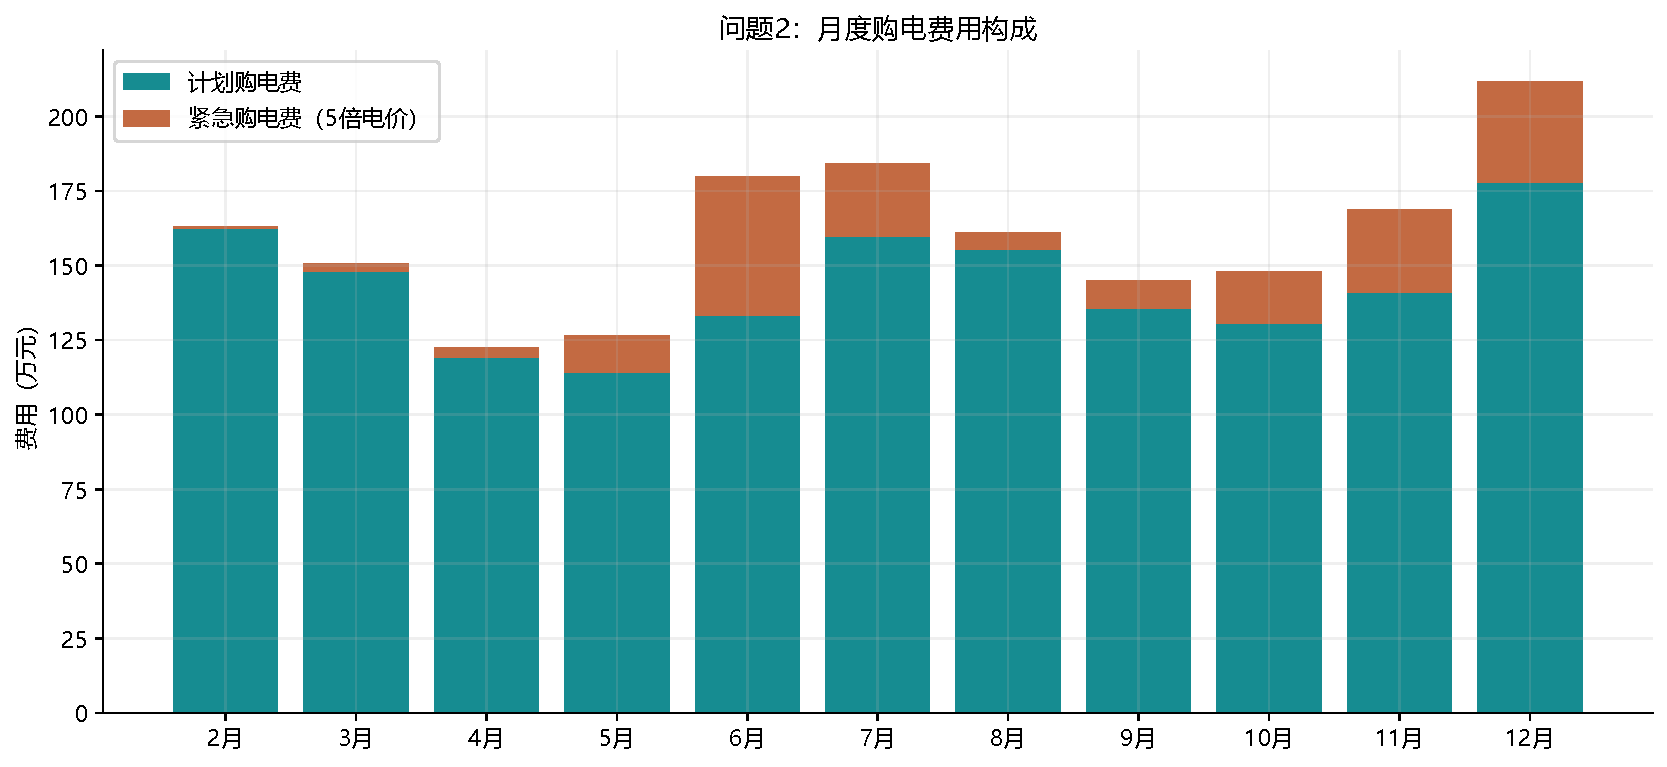
\includegraphics[width=.94\textwidth]{figures/q2_monthly.pdf}
\caption{问题二的月度计划费用与紧急费用}\end{figure}
风险来自历史场景对当前净负荷的覆盖不足。增加备购可以减少紧急费用，却可能扩大已支付合同的供能富余，因此需要联合权衡。与确定性均值、分位数及风险规避方法的同信息对照见后文，不能仅凭本模型可行就宣称其实际费用在所有策略中最低。
\FloatBarrier
